% =============================================================================
% Chapter 5: Game Mechanisms
% מנגנוני המשחק
% NEW CHAPTER - Detailed game mechanics, assignment tables, and failure handling
% =============================================================================

\documentclass[../master/main.tex]{subfiles}

\begin{document}

\setcounter{chapter}{4}
\hebrewchapter{מנגנוני המשחק}
\hebrewchapterlabel{chap:game-mechanisms}

\par\needspace{5\baselineskip}
\hebrewsection{מבוא}

פרק זה מפרט את המנגנונים הטכניים של מערכת המשחקים: טבלת ההקצאות, פורמט מזהה המשחק, חלונות הזמנים, וטיפול בתקלות טכניות.

\par\needspace{4\baselineskip}
\hebrewsubsection{מטרות הפרק}

בסיום פרק זה, תבינו:
\begin{itemize}
    \item את מבנה טבלת ההקצאות ואופן יצירתה
    \item את פורמט מזהה המשחק המורכב (\en{SSRRGGG})
    \item את חלונות הזמנים למשחקים
    \item את סוגי התקלות הטכניות וכלל \num{2}-\num{2}-\num{0}
    \item את פרוטוקול כוח עליון (\en{Force Majeure})
    \item את מחזור החיים של עונה ומחזור
\end{itemize}

% =============================================================================
\par\needspace{5\baselineskip}
\hebrewsection{טבלת ההקצאות (\en{Assignment Table})}
\label{sec:assignment-table}
% =============================================================================

\par\needspace{4\baselineskip}
\hebrewsubsection{מבנה הטבלה}

טבלת ההקצאות (\en{season\_assignments}) מכילה \num{180} שורות לכל עונה:
\begin{itemize}
    \item \num{60} משחקים × \num{3} משתתפים (שופט + \num{2} שחקנים) = \num{180} שורות
    \item \num{6} מחזורים × \num{10} משחקים למחזור = \num{60} משחקים
\end{itemize}

\begin{fancytable}{llH}{מבנה טבלת ההקצאות}
\label{tab:assignment-table-schema}
שדה & סוג & תיאור \\
\en{assignment\_id} & \en{SERIAL} & מזהה שורה ייחודי \\
\en{season\_id} & \en{VARCHAR(3)} & מזהה עונה (\en{S01}, \en{S02}) \\
\en{round\_id} & \en{VARCHAR(2)} & מספר מחזור (\en{01}--\en{06}) \\
\en{game\_id} & \en{VARCHAR(7)} & מזהה משחק מורכב (\en{SSRRGGG}) \\
\en{participant\_id} & \en{VARCHAR} & מזהה משתתף (\en{P-xxx} או \en{R-xxx}) \\
\en{role} & \en{ENUM} & תפקיד: \en{REFEREE}, \en{PLAYER\_A}, \en{PLAYER\_B} \\
\en{status} & \en{ENUM} & מצב: \en{ASSIGNED}, \en{CONFIRMED}, \en{COMPLETED} \\
\end{fancytable}

\par\needspace{4\baselineskip}
\hebrewsubsection{יצירת הטבלה}

הטבלה נוצרת אוטומטית בסגירת חלון ההרשמה:

\begin{figure}[htbp]
\centering
\begin{english}
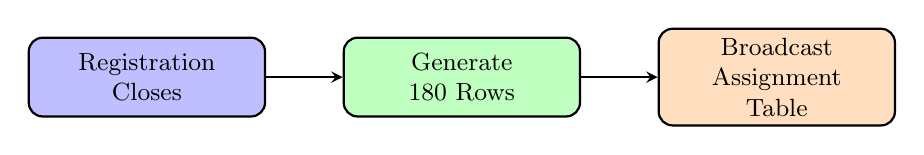
\begin{tikzpicture}[
    step/.style={draw, thick, fill=#1!25, minimum width=3cm, minimum height=1cm, rounded corners=5pt, align=center, font=\small},
    arrow/.style={->, thick, >=stealth}
]
    \node[step=blue] (reg) at (0,0) {Registration\\Closes};
    \node[step=green] (gen) at (4,0) {Generate\\180 Rows};
    \node[step=orange] (broad) at (8,0) {Broadcast\\Assignment\\Table};

    \draw[arrow] (reg) -- (gen);
    \draw[arrow] (gen) -- (broad);
\end{tikzpicture}
\end{english}
\caption{תהליך יצירת טבלת ההקצאות}
\label{fig:assignment-table-flow}
\end{figure}

\par\needspace{4\baselineskip}
\hebrewsubsection{הודעת שידור הקצאות}

מנהל הליגה שולח הודעת \en{BROADCAST\_ASSIGNMENT\_TABLE} לכל המשתתפים:

\needspace{10\baselineskip}
\begin{protocolbox}
הודעת \en{BROADCAST\_ASSIGNMENT\_TABLE} נשלחת פעם אחת בתחילת העונה. משתתף שלא קיבל את ההודעה יכול לבקש מסירה חוזרת באמצעות \en{REQUEST\_ASSIGNMENT\_TABLE}.
\end{protocolbox}

% =============================================================================
\par\needspace{5\baselineskip}
\hebrewsection{מזהה משחק מורכב (\en{SSRRGGG})}
\label{sec:game-id-composite}
% =============================================================================

\par\needspace{4\baselineskip}
\hebrewsubsection{פורמט המזהה}

מזהה המשחק הוא מחרוזת בת \num{7} ספרות בפורמט \en{SSRRGGG}:

\begin{fancytable}{cHlH}{מבנה מזהה משחק מורכב}
\label{tab:game-id-format}
מיקום & תווים & שדה & דוגמה \\
\en{1-2} & \en{SS} & מזהה עונה & \en{01} = עונה א' \\
\en{3-4} & \en{RR} & מספר מחזור & \en{03} = מחזור \num{3} \\
\en{5-7} & \en{GGG} & מספר משחק במחזור & \en{007} = משחק \num{7} \\
\end{fancytable}

\par\needspace{4\baselineskip}
\hebrewsubsection{דוגמאות פירוק}

\begin{fancytable}{lHHH}{דוגמאות לפירוק מזהה משחק}
\label{tab:game-id-examples}
מזהה & עונה & מחזור & משחק \\
\en{0101001} & עונה א' (\en{S01}) & מחזור \num{1} & משחק \num{1} \\
\en{0103007} & עונה א' (\en{S01}) & מחזור \num{3} & משחק \num{7} \\
\en{0206010} & עונה ב' (\en{S02}) & מחזור \num{6} & משחק \num{10} \\
\end{fancytable}

\par\needspace{4\baselineskip}
\hebrewsubsection{קוד פירוק מזהה}

\begin{english}
\begin{pythonbox}[\hebtitle{פירוק מזהה משחק}]
def parse_game_id(game_id: str) -> dict:
    """Parse SSRRGGG format into components."""
    if len(game_id) != 7 or not game_id.isdigit():
        raise ValueError(f"Invalid game_id: {game_id}")

    return {
        "season_id": f"S{game_id[0:2]}",   # SS -> S01
        "round_id": int(game_id[2:4]),      # RR -> 1-6
        "game_num": int(game_id[4:7])       # GGG -> 1-10
    }

# Example: parse_game_id("0103007")
# Returns: {"season_id": "S01", "round_id": 3, "game_num": 7}
\end{pythonbox}
\end{english}

% =============================================================================
\par\needspace{5\baselineskip}
\hebrewsection{חלונות זמנים למשחקים}
\label{sec:calendar-windows}
% =============================================================================

\par\needspace{4\baselineskip}
\hebrewsubsection{ימים ושעות}

משחקי הליגה מתקיימים בחלונות זמן קבועים:

\begin{fancytable}{Hcc}{חלונות זמנים למשחקים}
\label{tab:calendar-windows}
יום & שעת פתיחה (\en{GMT}) & שעת סגירה (\en{GMT}) \\
שלישי & \en{18:30} & \en{22:00} \\
חמישי & \en{18:30} & \en{22:00} \\
\end{fancytable}

\par\needspace{4\baselineskip}
\hebrewsubsection{תקופת חסד (\en{Grace Period})}

המערכת מעניקה תקופת חסד של \num{15} דקות:

\begin{itemize}
    \item \textbf{לפני פתיחה} --- משחק שהתחיל עד \num{15} דקות לפני \en{18:30} תקף
    \item \textbf{אחרי סגירה} --- משחק שהתחיל לפני \en{21:45} יכול להמשיך עד \en{22:00}
\end{itemize}

\par\needspace{4\baselineskip}
\hebrewsubsection{לוגיקת בדיקת זמן}

\begin{english}
\begin{pythonbox}[\hebtitle{בדיקת חלון זמן}]
def can_start_new_game(current_time: datetime) -> bool:
    """Check if new game can start in current time window."""
    # Check day of week (Tuesday=1, Thursday=3)
    if current_time.weekday() not in [1, 3]:
        return False

    # Check time window (18:30-22:00 GMT)
    start_time = current_time.replace(hour=18, minute=30)
    end_time = current_time.replace(hour=22, minute=0)

    return start_time <= current_time <= end_time
\end{pythonbox}
\end{english}

% =============================================================================
\par\needspace{5\baselineskip}
\hebrewsection{טיפול בתקלות טכניות}
\label{sec:technical-failures}
% =============================================================================

\par\needspace{4\baselineskip}
\hebrewsubsection{ארבעה סוגי תקלות}

המערכת מזהה ארבעה סוגי תקלות טכניות:

\begin{fancytable}{lHH}{סוגי תקלות טכניות}
\label{tab:failure-types}
סוג & תיאור & טריגר \\
\en{REFEREE\_NO\_SHOW} & שופט לא הגיע & אין תגובה להקצאה \\
\en{REFEREE\_ABANDONMENT} & שופט נטש משחק & אין תגובה באמצע משחק \\
\en{PLAYER\_NO\_SHOW} & שחקן לא הגיע & אין תגובה להזמנה \\
\en{GAME\_TIMEOUT} & המשחק חרג מזמן & חריגה ממגבלת \num{30} דקות \\
\end{fancytable}

\par\needspace{4\baselineskip}
\hebrewsubsection{כלל \num{2}-\num{2}-\num{0}}

בכל תקלה טכנית, המערכת מחילה ניקוד אוטומטי:

\needspace{10\baselineskip}
\begin{scoringbox}
\textbf{כלל \num{2}-\num{2}-\num{0}:}
\begin{itemize}
    \item שחקן א' מקבל \textbf{\num{2} נקודות}
    \item שחקן ב' מקבל \textbf{\num{2} נקודות}
    \item השופט מקבל \textbf{\num{0} נקודות}
\end{itemize}

הכלל חל כאשר המשחק לא הושלם בשל תקלה טכנית, ללא קשר לגורם התקלה.
\end{scoringbox}

\par\needspace{4\baselineskip}
\hebrewsubsection{תרשים טיפול בתקלות}

\begin{figure}[htbp]
\centering
\begin{english}
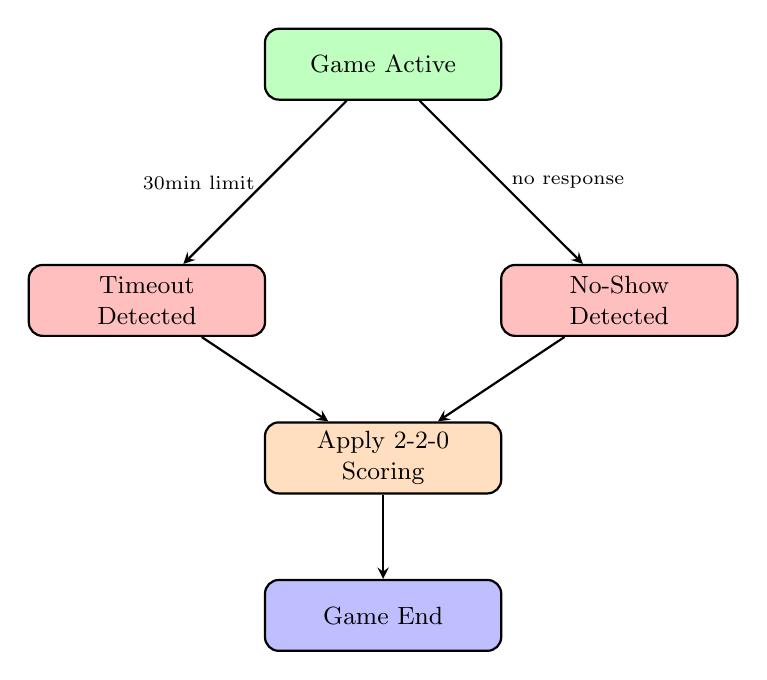
\begin{tikzpicture}[
    state/.style={draw, thick, fill=#1!25, minimum width=3cm, minimum height=0.9cm, rounded corners=5pt, align=center, font=\small},
    arrow/.style={->, thick, >=stealth}
]
    \node[state=green] (active) at (0,3) {Game Active};
    \node[state=red] (timeout) at (-3,0) {Timeout\\Detected};
    \node[state=red] (noshow) at (3,0) {No-Show\\Detected};
    \node[state=orange] (scoring) at (0,-2) {Apply 2-2-0\\Scoring};
    \node[state=blue] (end) at (0,-4) {Game End};

    \draw[arrow] (active) -- (timeout) node[midway, left, font=\scriptsize] {30min limit};
    \draw[arrow] (active) -- (noshow) node[midway, right, font=\scriptsize] {no response};
    \draw[arrow] (timeout) -- (scoring);
    \draw[arrow] (noshow) -- (scoring);
    \draw[arrow] (scoring) -- (end);
\end{tikzpicture}
\end{english}
\caption{תהליך טיפול בתקלות טכניות עם ניקוד \num{2}-\num{2}-\num{0}}
\label{fig:failure-handling-flow}
\end{figure}

% =============================================================================
\par\needspace{5\baselineskip}
\hebrewsection{פרוטוקול כוח עליון (\en{Force Majeure})}
\label{sec:force-majeure}
% =============================================================================

\par\needspace{4\baselineskip}
\hebrewsubsection{מהו כוח עליון?}

כוח עליון הוא מצב שבו תקלה חיצונית מונעת המשך תקין של המשחק:

\begin{itemize}
    \item תקלת רשת כללית
    \item בעיה בשרתי \en{Gmail}
    \item תקלה במערכת מנהל הליגה
    \item נסיבות חריגות אחרות
\end{itemize}

\par\needspace{4\baselineskip}
\hebrewsubsection{תהליך הבקשה}

\begin{figure}[htbp]
\centering
\begin{english}
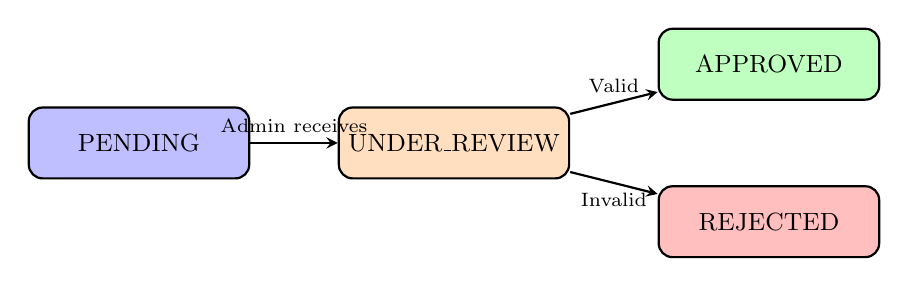
\begin{tikzpicture}[
    state/.style={draw, thick, fill=#1!25, minimum width=2.8cm, minimum height=0.9cm, rounded corners=5pt, align=center, font=\small},
    arrow/.style={->, thick, >=stealth}
]
    \node[state=blue] (pending) at (0,2) {PENDING};
    \node[state=orange] (review) at (4,2) {UNDER\_REVIEW};
    \node[state=green] (approved) at (8,3) {APPROVED};
    \node[state=red] (rejected) at (8,1) {REJECTED};

    \draw[arrow] (pending) -- (review) node[midway, above, font=\scriptsize] {Admin receives};
    \draw[arrow] (review) -- (approved) node[midway, above, font=\scriptsize] {Valid};
    \draw[arrow] (review) -- (rejected) node[midway, below, font=\scriptsize] {Invalid};
\end{tikzpicture}
\end{english}
\caption{מכונת מצבים של בקשת כוח עליון}
\label{fig:force-majeure-states}
\end{figure}

\par\needspace{4\baselineskip}
\hebrewsubsection{הודעות כוח עליון}

\begin{fancytable}{lHHc}{הודעות כוח עליון}
\label{tab:force-majeure-messages}
סוג הודעה & מאת & אל & מועד \\
\en{FORCE\_MAJEURE\_REQUEST} & שופט/שחקן & מנהל & -- \\
\en{FORCE\_MAJEURE\_DECISION} & מנהל & מבקש & \en{24h} \\
\en{FORCE\_MAJEURE\_RESULT} & מנהל & כל המשתתפים & -- \\
\end{fancytable}

\needspace{10\baselineskip}
\begin{warningbox}[\hebtitle{שימוש במשורה}]
בקשות כוח עליון נבדקות בקפידה. שימוש לרעה במנגנון (למשל, לכיסוי על תקלה בקוד) עלול לגרום לדחיית בקשות עתידיות ולהורדת ציון.
\end{warningbox}

\par\needspace{4\baselineskip}
\hebrewsubsection{פורמט בקשת כוח עליון}

הסוכן שולח בקשת כוח עליון בפורמט הבא:

\begin{english}
\begin{pythonbox}[\hebtitle{בקשת כוח עליון}]
{
  "message_type": "FORCE_MAJEURE_REQUEST",
  "payload": {
    "game_id": "0103005",
    "reason_category": "MEDICAL",
    "description": "Player hospitalized",
    "evidence_urls": ["url1", "url2"],
    "requested_action": "RESCHEDULE"
  },
  "correlation_id": "uuid-for-tracking"
}
\end{pythonbox}
\end{english}

\begin{fancytable}{lH}{קטגוריות סיבה לכוח עליון}
\label{tab:force-majeure-reasons}
קטגוריה & תיאור \\
\en{MEDICAL} & מצב רפואי מתועד \\
\en{TECHNICAL\_INFRASTRUCTURE} & תקלה בתשתית (חשמל, אינטרנט) \\
\en{PERSONAL\_EMERGENCY} & מקרה חירום אישי \\
\en{NATURAL\_DISASTER} & אסון טבע \\
\en{MILITARY\_SERVICE} & שירות מילואים \\
\end{fancytable}

\begin{fancytable}{lH}{פעולות מבוקשות}
\label{tab:force-majeure-actions}
פעולה & משמעות \\
\en{RESCHEDULE} & קביעת מועד חדש למשחק \\
\en{CANCEL} & ביטול המשחק (ללא ניקוד) \\
\en{SCORE\_ADJUSTMENT} & התאמת הניקוד ידנית \\
\end{fancytable}

% =============================================================================
\par\needspace{5\baselineskip}
\hebrewsection{פרוטוקול בקשת הארכה}
\label{sec:extension-protocol}
% =============================================================================

כאשר סוכן צופה שלא יספיק לעמוד בדדליין, הוא יכול לבקש הארכה \textbf{לפני} שהזמן יפוג.

\par\needspace{4\baselineskip}
\hebrewsubsection{מתי לבקש הארכה}

\begin{itemize}
\item זמן התגובה הנדרש עומד לפוג
\item הסוכן מזהה שהעיבוד יארך יותר מהצפוי
\item תקלה זמנית מונעת תגובה מיידית
\end{itemize}

\begin{warningbox}[\hebtitle{בקשה מוקדמת}]
יש לשלוח בקשת הארכה \textbf{לפני} שפג תוקף הדדליין. בקשה שנשלחת לאחר הדדליין תידחה אוטומטית.
\end{warningbox}

\par\needspace{4\baselineskip}
\hebrewsubsection{זיהוי חלונות זמן באמצעות \en{Google Calendar}}

\begin{notebox}[\hebtitle{תוכנית גיבוי}]
במקרה שמנהל הליגה אינו זמין או חווה תקלה טכנית, הסוכן יכול לזהות את פתיחת חלון הזמן באמצעות אירועי \en{Google Calendar} המשותף. לוח השנה מכיל את כל האירועים הקריטיים:
\begin{itemize}
    \item \en{REG\_SEASON} --- חלון רישום סוכנים (\en{18:30--18:45})
    \item \en{ROUND\_1} עד \en{ROUND\_6} --- מחזורי משחקים
    \item \en{FINAL\_RESULTS} --- פרסום תוצאות (\en{21:45--22:00})
\end{itemize}
כאשר הסוכן מזהה אירוע יומן ללא הודעה מקבילה ממנהל הליגה, עליו לפעול באופן יזום ולשלוח את ההודעה המתאימה (רישום/אישור הצטרפות וכו').
\end{notebox}

\par\needspace{4\baselineskip}
\hebrewsubsection{פורמט בקשת הארכה}

\begin{english}
\begin{pythonbox}[\hebtitle{בקשת הארכה}]
{
  "message_type": "EXTENSION_REQUEST",
  "payload": {
    "original_message_id": "uuid-of-original",
    "original_message_type": "GAME_JOIN_ACK",
    "reason": "Processing complex game state",
    "requested_extension_seconds": 120
  },
  "correlation_id": "uuid-for-tracking"
}
\end{pythonbox}
\end{english}

\par\needspace{4\baselineskip}
\hebrewsubsection{תגובת השרת}

השרת מגיב עם \en{RESPONSE\_EXTENSION}:

\begin{english}
\begin{pythonbox}[\hebtitle{תגובת הארכה}]
{
  "message_type": "RESPONSE_EXTENSION",
  "payload": {
    "status": "APPROVED",
    "new_deadline": "2025-01-15T19:05:00Z",
    "extension_seconds": 120,
    "reason": "Extension granted"
  },
  "correlation_id": "uuid-from-request"
}
\end{pythonbox}
\end{english}

\begin{notebox}[\hebtitle{סטטוס תגובה}]
שדה \en{status} יכול להיות \en{"APPROVED"} (הארכה אושרה) או \en{"DENIED"} (הארכה נדחתה).
\end{notebox}

\begin{fancytable}{lHH}{טיפול בתגובת הארכה}
\label{tab:extension-handling}
סטטוס & פעולה נדרשת & הערות \\
\en{APPROVED} & השתמש בדדליין החדש & המשך עיבוד ושלח תגובה \\
\en{DENIED} & שלח תגובה מיידית & או קבל \en{REJECTION\_NOTIFICATION} \\
\end{fancytable}

\par\needspace{4\baselineskip}
\hebrewsubsection{מימוש מומלץ}

\begin{english}
\begin{pythonbox}[\hebtitle{מנהל הארכות}]
class ExtensionManager:
    async def request_extension_if_needed(
        self,
        original_msg: dict,
        deadline: datetime,
        processing_estimate: float
    ) -> bool:
        """Request extension if we won't make deadline."""
        time_remaining = (deadline - datetime.now()).total_seconds()

        if time_remaining < processing_estimate + 30:
            response = await self.send_extension_request(
                original_msg,
                requested_seconds=120
            )
            return response.get("status") == "APPROVED"
        return True
\end{pythonbox}
\end{english}

% =============================================================================
\par\needspace{5\baselineskip}
\hebrewsection{מחזור חיים של עונה}
\label{sec:season-lifecycle}
% =============================================================================

\par\needspace{4\baselineskip}
\hebrewsubsection{מצבי העונה}

\begin{figure}[htbp]
\centering
\begin{english}
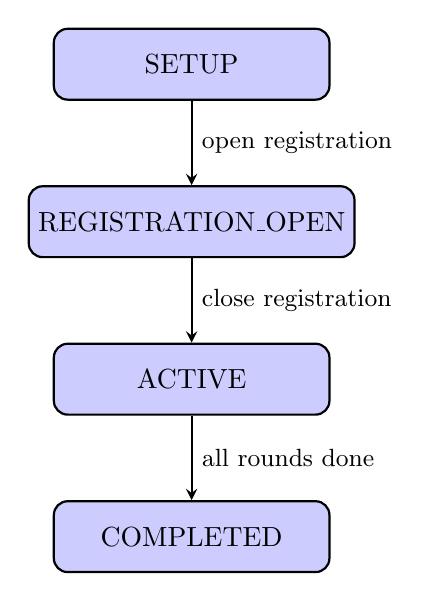
\begin{tikzpicture}[
    state/.style={draw, thick, fill=blue!20, rounded corners=5pt, minimum width=3.5cm, minimum height=0.9cm, align=center},
    arrow/.style={->, thick, >=stealth}
]
    \node[state] (setup) at (0,4) {SETUP};
    \node[state] (reg) at (0,2) {REGISTRATION\_OPEN};
    \node[state] (active) at (0,0) {ACTIVE};
    \node[state] (completed) at (0,-2) {COMPLETED};

    \draw[arrow] (setup) -- (reg) node[midway, right, font=\small] {open registration};
    \draw[arrow] (reg) -- (active) node[midway, right, font=\small] {close registration};
    \draw[arrow] (active) -- (completed) node[midway, right, font=\small] {all rounds done};
\end{tikzpicture}
\end{english}
\caption{מכונת מצבים של עונה}
\label{fig:season-state-machine}
\end{figure}

\begin{fancytable}{lHH}{מצבי עונה ומעברים}
\label{tab:season-states}
מצב & תיאור & טריגר למעבר הבא \\
\en{SETUP} & הכנה לעונה & פתיחת הרשמה \\
\en{REGISTRATION\_OPEN} & חלון הרשמה פתוח & סגירת חלון ההרשמה \\
\en{ACTIVE} & העונה פעילה & סיום כל \num{6} המחזורים \\
\en{COMPLETED} & העונה הסתיימה & -- \\
\end{fancytable}

% =============================================================================
\par\needspace{5\baselineskip}
\hebrewsection{מחזור חיים של מחזור משחקים}
\label{sec:round-lifecycle}
% =============================================================================

\par\needspace{4\baselineskip}
\hebrewsubsection{מצבי המחזור}

\begin{fancytable}{lHH}{מצבי מחזור משחקים}
\label{tab:round-states}
מצב & תיאור & הודעה מופעלת \\
\en{SCHEDULED} & המחזור מתוכנן & -- \\
\en{IN\_PROGRESS} & המחזור פעיל & \en{ROUND\_STARTED} \\
\en{COMPLETED} & המחזור הסתיים & \en{ROUND\_ENDED} \\
\end{fancytable}

\par\needspace{4\baselineskip}
\hebrewsubsection{הודעות מחזור}

מנהל הליגה שולח הודעות בתחילת ובסוף כל מחזור:

\begin{itemize}
    \item \textbf{\en{BROADCAST\_ROUND\_START}} --- הודעה על תחילת מחזור עם רשימת המשחקים
    \item \textbf{\en{BROADCAST\_ROUND\_END}} --- סיכום תוצאות המחזור
    \item \textbf{\en{BROADCAST\_SEASON\_STANDINGS}} --- טבלת דירוג מעודכנת
\end{itemize}

% =============================================================================
\par\needspace{5\baselineskip}
\hebrewsection{סיכום}
% =============================================================================

פרק זה הציג את מנגנוני המשחק המרכזיים:

\begin{itemize}
    \item \textbf{טבלת הקצאות} --- \num{180} שורות (\num{60} משחקים × \num{3} משתתפים)
    \item \textbf{מזהה משחק} --- פורמט \en{SSRRGGG} (עונה-מחזור-משחק)
    \item \textbf{חלונות זמנים} --- שלישי/חמישי \en{18:30-22:00 GMT}
    \item \textbf{תקלות טכניות} --- \num{4} סוגים עם ניקוד \num{2}-\num{2}-\num{0}
    \item \textbf{כוח עליון} --- \en{PENDING → UNDER\_REVIEW → APPROVED/REJECTED}
    \item \textbf{מחזור חיי עונה} --- \en{SETUP → REGISTRATION → ACTIVE → COMPLETED}
    \item \textbf{מחזור חיי מחזור} --- \en{SCHEDULED → IN\_PROGRESS → COMPLETED}
\end{itemize}

בפרק הבא נעסוק במימוש המעשי של הסוכנים.

\end{document}
